\documentclass[
    11pt,
    a4paper,
    english,
    brazil
    ]{article}

\usepackage[utf8]{inputenc} %Colocar acento
\usepackage[T1]{fontenc}    %Saída boa para impressora
\usepackage{indentfirst}    %Coloca espaço no primeiro paragrafo
\usepackage[brazil]{babel}  %Trata o texto como português
\usepackage[top=1cm, left=2cm, right=1.5cm, bottom=1.5cm]{geometry} %Arruma borda
\usepackage{graphicx}   %Pacote gerencia imagem
\usepackage{float}      %pacote que força o local de figuras, tabelas, etc.
\usepackage{xcolor}     %pacote de cores
\usepackage{lmodern}    % Usa a fonte Latin Modern	
\usepackage{hyperref}   %Link itens no texto
\usepackage[normalem]{ulem}
\useunder{\uline}{\ul}{}
\usepackage{longtable}


\title{Instruções para elaborar uma estratégia de transformação digital}
\author{Elaborado por Renan da Silva Marques (UFABC)/2022}
\date{}

\pagenumbering{empty} %Remover números das páginas

\begin{document}
\maketitle

Este documento visa instruir a criação de uma estratégia de transformação digital, independente da organização e contexto. A figura \ref{fig:mapETD} apresenta o diagrama do processo, que deve ser interpretado de maneira ordenada:

\begin{figure}[!htpb]
    \centering
    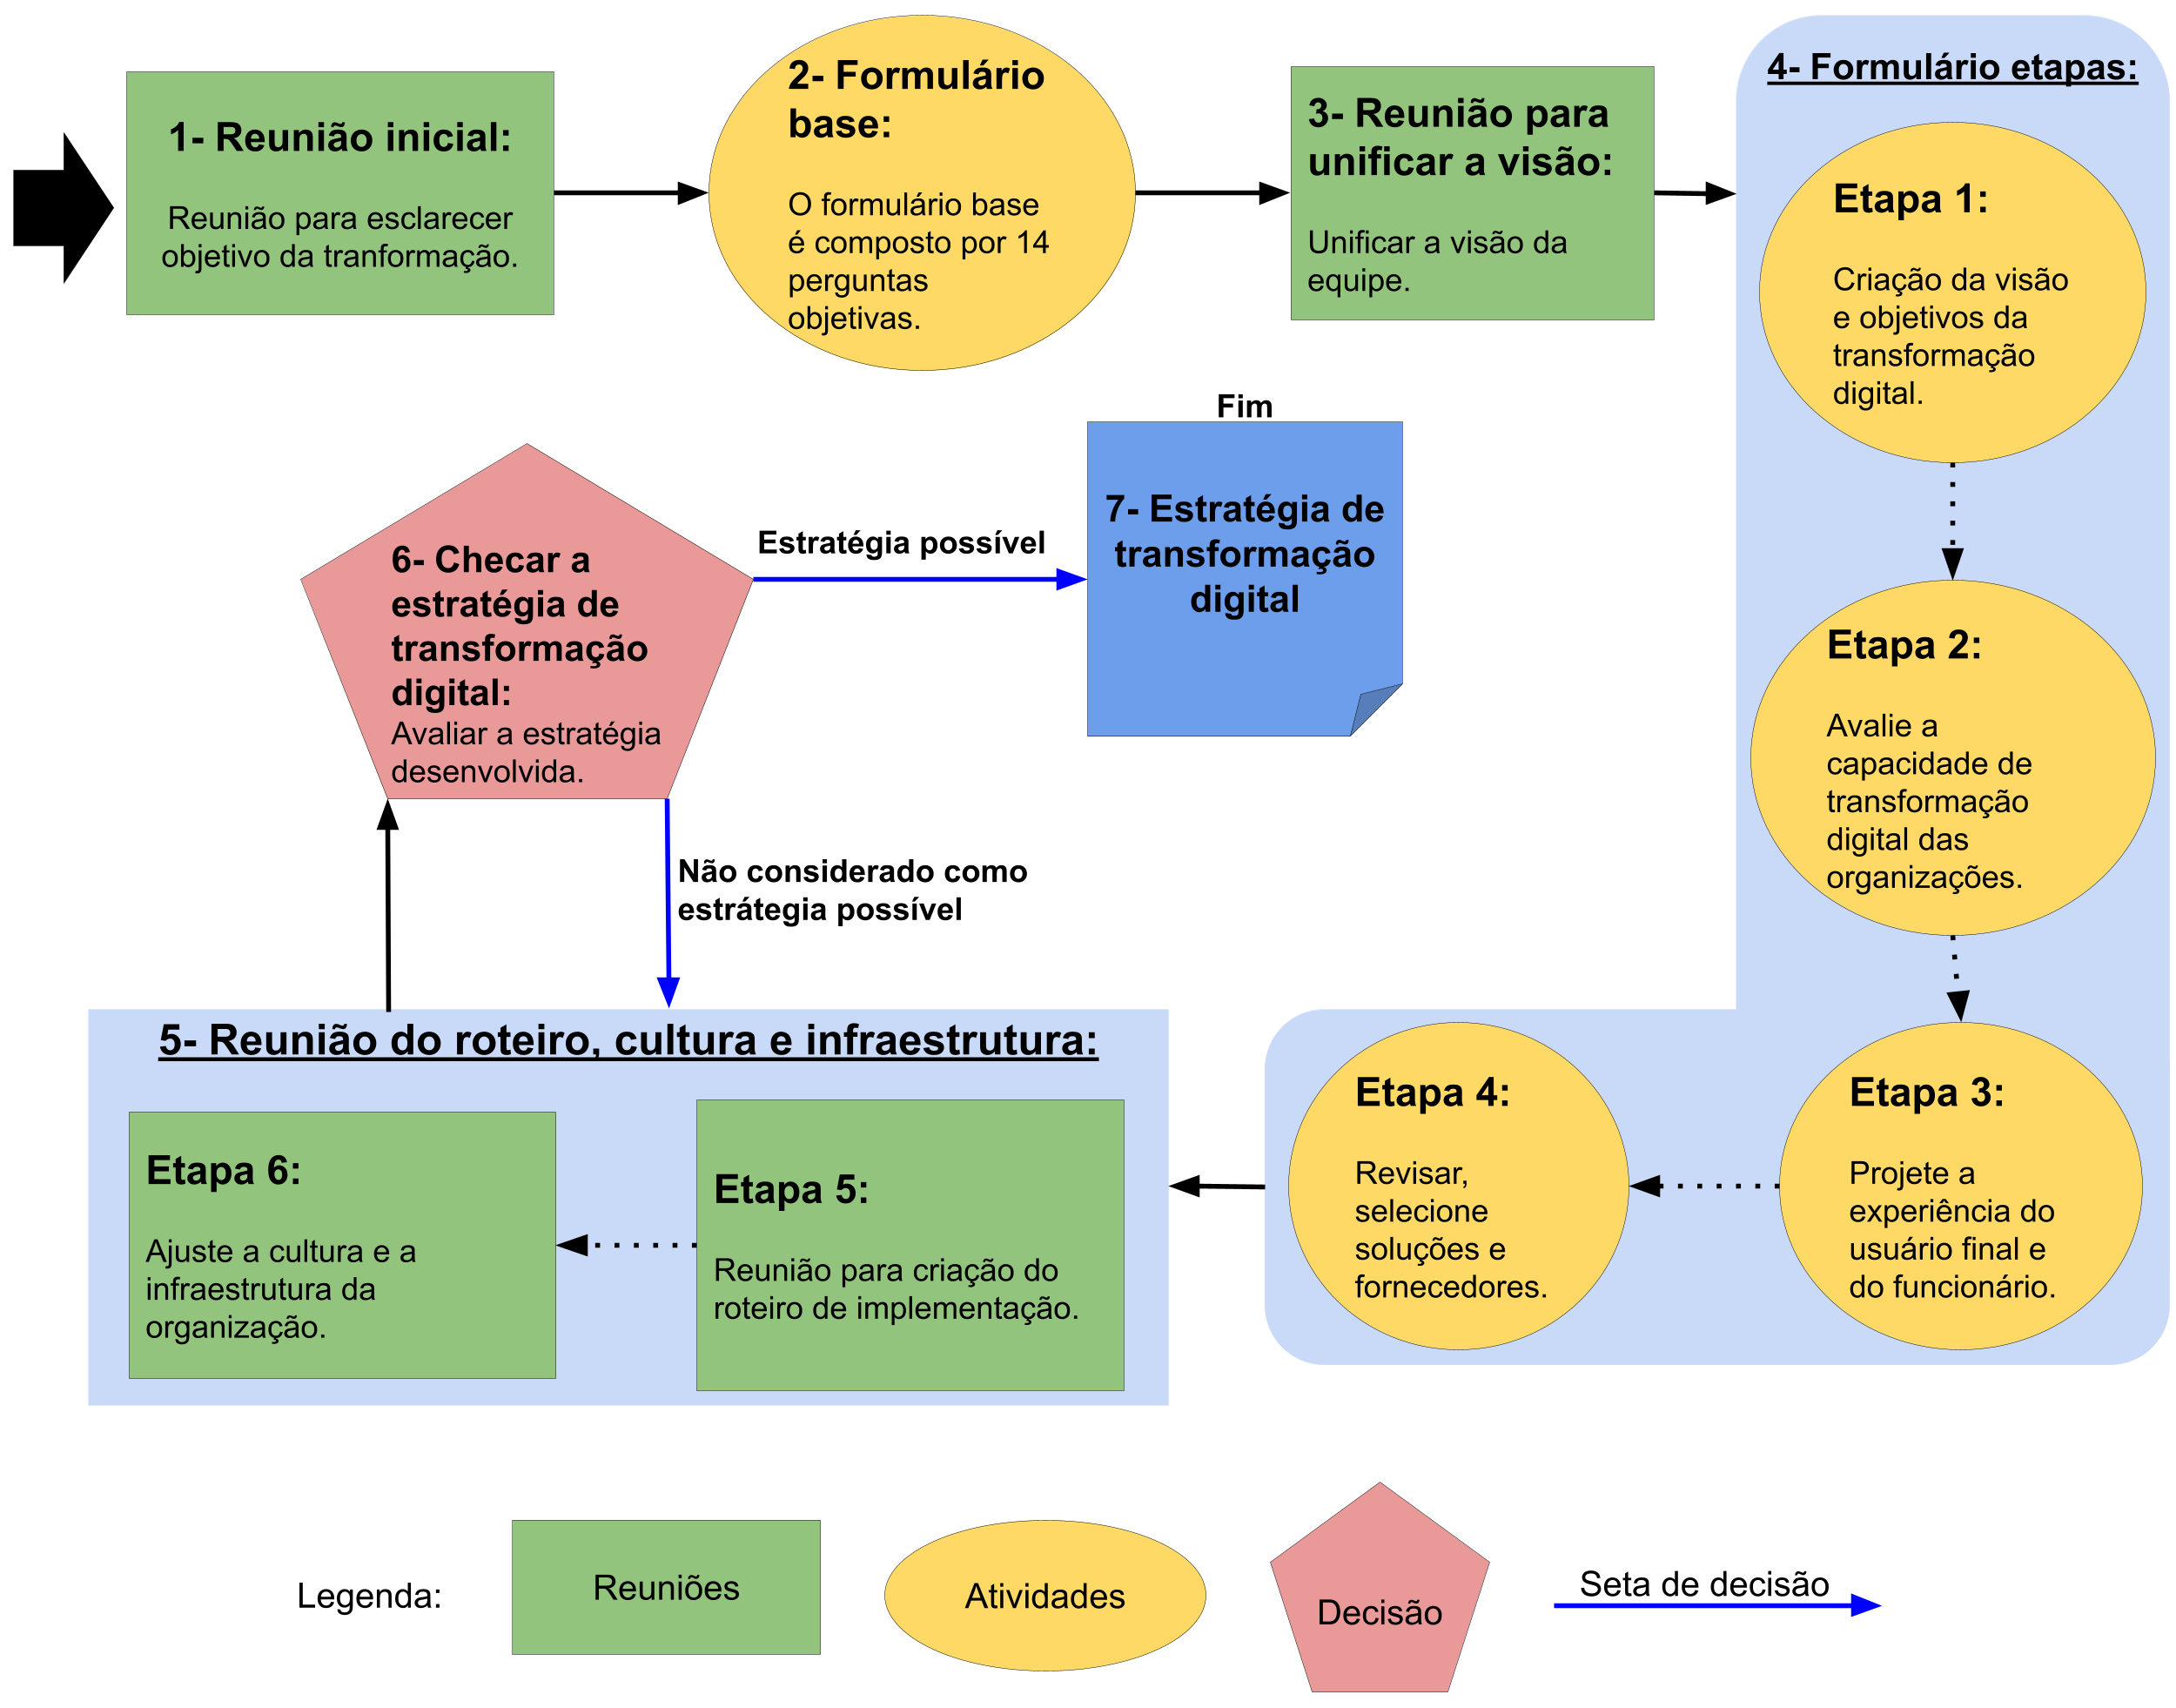
\includegraphics[scale=0.18]{figuras/mapETD.png}
    \caption{Diagrama do processo para elaborar uma estratégia de transformação digital.}
    \label{fig:mapETD}
\end{figure}



\section{Reunião inicial}\label{sec:reuniaoInicial}

O primeiro passo é realizar uma reunião, em que devem participar todas as partes interessadas. A reunião deve abordar minimamente os seguintes itens:

\begin{itemize}
    \item O que é a transformação digital e a sua importância.
    \item Estratégia de transformação digital e a sua importância.
    \item Como devem ocorrer as etapas seguintes e os objetivos.
    \item Esclarecer qualquer outra dúvida que os participantes tenham inicialmente.
\end{itemize}

O objetivo desta etapa é garantir que todos os participantes estejam cientes do processo que se inicia.



\section{Formulário base}\label{sec:atividadeFormBase}

A segunda etapa, tem o objetivo de sumarizar todas as características que devem ser buscadas pela organização, durante a transformação digital. Todos os participantes devem preencher o formulário base de maneira individual.



\section{Reunião para unificar a visão}

A reunião para unificar a visão, tem o objetivo de consolidar em uma única perspectiva, os objetivos da transformação digital definidas de maneira individual na atividade "\nameref{sec:atividadeFormBase}". Assim, partindo de uma única sumarização, todas as próximas atividades, mesmo que diferentes, tendem a chegar em um mesmo objetivo.

Na reunião para unificar a visão, um dos participantes deve ficar responsável por preencher um novo formulário base, através do consenso entre todos os participantes. Para cada pergunta do formulário, todos os participantes devem expor suas respostas, e o(s) participante(s) que não escolheu a resposta da maioria, deve expor o motivo de sua escolha. Se ainda sim, a maioria não concordar, a resposta da maioria deve ser marcado no formulário base.

Ao final da reunião, o formulário base preenchido deve ser disponibilizado para todos os participantes, e está sumarização dos objetivos deve ser considerado para as atividades subsequentes.


\section{Formulário de atividades}\label{sec:formAtividade}

O formulário de atividades é composto por 4 etapas, que devem ser realizadas de maneira individual e descritas com o máximo de detalhes possível. As atividades da etapa englobam objetivos, futuras experiências com clientes e funcionários, aspectos da infraestrutura, capacidade e flexibilidade da organização, maneiras de simplificar o trabalho dos funcionários, facilitar o acesso do cliente, e por fim, deve-se realizar uma seleção de soluções e de fornecedores.

Todas as atividades realizadas pelo "\nameref{sec:formAtividade}" deve ser entregue, ou acessada pelo responsável da estratégia de transformação digital, definido pelo "\nameref{sec:formBase}". Onde o mesmo deve realizar uma compilação dos resultados, e transcrever os objetivos específicos, as capacidades, experiência de clientes e funcionários e potenciais soluções e fornecedores.

\section{Reunião do roteiro, cultura e infraestrutura}\label{sec:reuniaoRoteiroCulturaInfraestrutura}

A compilação dos resultados do "\nameref{sec:formEtapas}" devem ser disponibilizado para todos os participantes antes da "\nameref{sec:reuniaoRoteiroCulturaInfraestrutura}". Duas etapas devem ser realizadas nesta reunião, sendo elas, a criação do roteiro de implementação (Etapa 5), e também a identificação de ajustes na cultura e infraestrutura da organização (Etapa 6). O responsável por elaborar a estrategia deve realizar anotações sobre cada atividade, para que posteriormente complete a documentação contendo a estratégia de transformação digital.\\

A etapa 5 é composta pelas seguintes atividades:
\begin{itemize}
    \item De acordo com as etapas anteriores, descreva o primeiro passo/preparação para a implementação.
    
    \item Descreva os passos da implementação em si.
    
    \item Descreva os passos no âmbito financeiro da implementação.
    
    \item Descreva também o passo final/finalização da implementação.\\
\end{itemize}

E a etapa 6, composta pelas seguintes atividades:
\begin{itemize}
    \item Descreva ajustes da cultura que devem ser construídas ou adaptadas na organização.
    
    \item Descreva modificações que devem ocorrer na infraestrutura da organização.
    
    \item Descreva funções de um equipe dedicada, juntamente com o nome de um possível especialista ou "a contratar", quando a organização não tem um colaborador apto para uma nova função.
    
    \item Para ajustar a cultura e a infraestrutura, quais recursos financeiros serão necessários?
\end{itemize}



\section{Checagem da estratégia}\label{sec:checagemDaEstrategia}

Esta etapa deve ser realizada pelos idealizadores da organização, que consiga identificar implementações que podem não ser viáveis para a organização, assim como também identificar problemas no plano e se as soluções selecionadas possam, de alguma maneira, não serem disponibilizadas para a organização.


\section{Finalização}

Por fim, um único documento contendo o plano e instruções, que compilados se caracterizam em uma estratégia de transformação digital, deve ser apresentado para toda a organização. Estratégia essa que deve ser iniciada quanto antes, garantindo assim a validade e eficiência do plano elaborado.

\begin{center}
    \textbf{\huge Anexos e instruções de uso}
\end{center}

Os anexos devem ser utilizados pelo responsável em conduzir a elaboração da transformação digital, com o intuito de introduzir conhecimentos mínimos necessários para conduzir as reuniões.

\section*{Definições para a etapa \ref{sec:reuniaoInicial}}

A primeira atividade é composta pela reunião inicial, onde alguns itens devem ser introduzidos para os participantes do processo para elaborar uma estratégia de transformação digital. Breve explicações podem ser observadas a seguir:

\begin{itemize}
    \item \textbf{Transformação digital:}\\
    Transformação digital é mais que apenas implementar novas tecnologia, investir em ferramentas digitais ou atualizar sistemas existentes, mas é também mudar o modelo de negócio, da produção até o cliente final. É composta pelas fases de digitização (Procedimentos básicos, como, por exemplo, converter um livro em um documento digital.), digitalização (Indo além e permitindo, por exemplo, novas interações, figuras animadas ou até vídeo.) e a própria transformação digital (Podendo englobar todos os itens anteriores, mas que tem a finalidade de mudar a forma de negócio, como, por exemplo, a compra de livros de maneira virtual, difundindo das tradicionais bibliotecas.), que por fim normalmente envolve cinco elementos:
    
    \begin{figure}[!htpb]
        \centering
        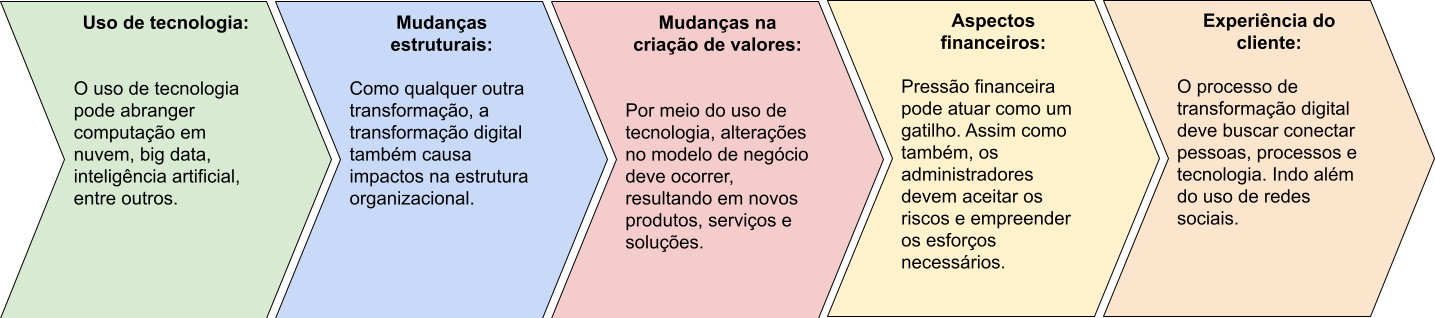
\includegraphics[scale=0.32]{figuras/elementosTD.png}
        \caption{Elementos da transformação digital (elaborado pelo autor).}
        \label{fig:mapETD}
    \end{figure}
    
    \item \textbf{Importância da transformação digital:}\\
    A evolução da tecnologia é um caminho natural para a evolução humana, mudando maneiras de trabalhar e até de se divertir, a tal ponto de que diversos serviços se tornaram majoritariamente oferecidos por meios digitais, como sites e aplicativos. Por tanto, tornando a transformação digital um elemento importante a não ser negligenciado pelas organizações, para que assim se mantenha relevante entre a ampla concorrência, além de que organizações de maior maturidade digital são mais flexíveis.
    
    \item \textbf{Estratégia de transformação digital:}\\
    Estratégia transformação digital consiste em um conjunto de planos previamente elaborados para auxiliar na implementação de tecnologias, de modo a obter sucesso para alcançar às dimensões de quatro itens da transformação digital (Uso de tecnologia, mudanças estruturais, mudanças na criação de valores e aspectos financeiros). Não deve ser interpretado como uma estratégia de TI, ou estratégia para implementar um determinado programa computacional, pois estratégia de transformação digital não deve ser tratada de maneira isolada.
    
    Tornar-se digitalmente maduro é um dos objetivos ao se desenvolver uma estratégia de transformação digital, logo, o planejamento deve incluir objetivos de médio e longo prazo.
    
    \item \textbf{Importância da estratégia de transformação digital:}\\
    Existem atualmente inúmeras possibilidades digitais, compostas por diversas complexidades que possibilitam passos equivocados, por isso, é de grande importância elaborar uma boa estratégia de transformação digital, dado que uma estratégia de transformação digital bem elaborada e clara, é de extrema importância para o sucesso geral de diversas implementações e avanços organizacionais.
    
    \item \textbf{Como as seguintes etapas vão ser conduzida:}\\
    Após a primeira etapa, composta pela reunião inicial, onde são realizadas explicações e esclarecimento do processo a se iniciar. As seguintes etapas devem ser executadas em suas respectivas ordens, além de que o acesso aos formulários também devem ser garantido.
    
    Os formulários estão disponibilizados no anexo "\nameref{sec:formBase}" e "\nameref{sec:formEtapas}", e podem ser disponibilizados de maneira física ou virtual, no entanto, ferramentas virtuais facilitam a apuração das respostas.
    
    Na etapa "\nameref{sec:checagemDaEstrategia}", caso seja definido que a estratégia não é possível, ou seja, identificada que a estratégia por algum motivo, seja técnico, financeiro, ou qualquer outro motivo que possa impedir a aplicação da mesma, todo o processo deve ser retornado para a etapa "\nameref{sec:reuniaoRoteiroCulturaInfraestrutura}", e novos ajustes devem ser conduzidos, de maneira a tornar a estratégia viável para a organização.
    
    Após a aprovação da estratégia de transformação digital pela etapa de "\nameref{sec:reuniaoRoteiroCulturaInfraestrutura}", o documento contendo a estratégia deve ser implementada em toda organização o mais breve possível, garantindo dessa maneira a validade da estratégia.
    
    
    \item \textbf{Dúvidas:}\\
    Dúvidas sobre próximas reuniões, e disponibilidade dos questionários devem ser esclarecidas.
\end{itemize}


\section*{Formulário base}\label{sec:formBase}

\textbf{Uso de tecnologia}\\

\underline{1 - Papel estratégico da TI}\\

\textit{Contextualização}

Algumas organizações podem naturalmente terem propensão a se transformarem digitalmente, seja pela área de atuação, ou o modelo de negócio que permite grandes modificações. Neste sentido, classifique o papel estratégico que o TI terá na sua organização, podendo ser ela facilitadora ou apoiadora:

- Facilitador: em algumas organizações é necessário um impulso inicial com o uso de uma nova tecnologia digital, desta maneira, facilitador é quando a transformação digital não ocorre naturalmente, sendo necessário um facilitador.

- Apoiar: em outras organizações, as transformações ocorrem naturalmente, e o uso de uma nova tecnologia tem o intuito de apoiar.\\

\textit{Pergunta}

Qual a importância que o TI terá em sua organização, para atingir os objetivos da transformação digital? Ou descreva outro papel que o TI terá na organização.

( ) Facilitador

( ) Apoiar

Outro:\\


\underline{2 - Quão ambiciosa sua organização é diante de novas tecnologias?}\\

\textit{Contextualização}

A ambição tecnológica está ligada com o quão inovadora, ou conservadora será sua organização diante das tecnologias a serem adotadas.

- Inovador: quando a organização quer ser autora de ideias inovadoras.

- Early adopter: quando a organização quer ser a primeira a testar e fornecerem comentários de novas tecnologias.

- Seguidor: quando se deseja ser mais conservador, e utilizar tecnologias já estabelecidas.\\

\textit{Pergunta}

Qual a ambição tecnológica será buscada pela sua organização? Ou descreva outra ambição.

( ) Inovador

( ) Early adopter

( ) Seguidor

Outro:\\

\textbf{Mudanças na criação de valor}\\

\underline{3 - Grau de diversificação digital?}\\

\textit{Contextualização}

A diversificação digital é como a organização pretende disponibilizar os produtos da organização, visando produtos atuais e produtos a serem disponibilizados ao decorrer da transformação digital:

- Canais de vendas eletrônicos: Mantendo produtos analógicos, apenas utilizando um canal para alcançar clientes.

- Mídia cruzada: Utiliza soluções digitais para armazenamento de dados.

- Mídia enriquecida: Armazenamento aprimorado, possibilitando por exemplos ferramentas de buscas.

- Plataformas de conteúdo: Possibilita trabalhar com os dados, como, por exemplo, minerar dados.

- Negócio ampliado: Possibilidade de criar valores organizacional e ampliando os produtos, por exemplo, gerando informações extras.

- Organização sem fins lucrativos: Quando a organização não tem o objetivo de gerar receita.\\


\textit{Pergunta}

Como sua organização pretende impulsionar as vendas digitais? Ou descreva outra diversificação.

( ) Canais de vendas eletrônicos

( ) Mídia cruzada

( ) Mídia enriquecida

( ) Plataformas de conteúdo

( ) Negócio ampliado

( ) Organização sem fins lucrativos

Outro(s):\\


\underline{4 - Criação de receita}\\

\textit{Contextualização}

A criação de receita tem o objetivo de definir meio para que a organização se mantenha financeiramente:

Utilizar soluções digitais, podem acarretar gastos adicionais. Desta maneira, a organização precisa definir maneiras para se manter financeiramente.


- Conteúdo pago: necessário pagamento para clientes acessarem o site.

- Freemium: conteúdos adicionais ou parte do site apenas para assinantes.

- Propaganda: site exibindo propagandas.

- Produtos complementares: Serviços/produtos extras, além do principal.\\


\textit{Pergunta}

Como a organização vai adaptar os produtos para gerar receita? Ou descreva outra adaptação.

( ) Conteúdo pago

( ) Freemium

( ) Propaganda

( ) Produtos complementares

Outro(s):\\

\underline{5 - Futuro escopo do negócio principal}\\

\textit{Contextualização}

A transformação digital altera o modelo de negócio, e em função aos artefatos da organização, o escopo do negócio principal precisa ser definido. Organizações podem desde gerar novos conteúdos, até mesmo fornecer uma plataforma para outras organizações.

- Criação de conteúdo: criar conteúdos novos.

- Agregação de conteúdo: juntar/concentrar conteúdos.

- Distribuição de conteúdo: fornecer suporte para distribuir o conteúdo.

- Gerenciamento de plataformas de conteúdo: fornecer suporte para a plataforma de conteúdo, para conseguir gerenciar os conteúdos.\\


\textit{Pergunta}

Qual o futuro escopo do negócio principal? Ou descreva outro escopo.

( ) Criação de conteúdo

( ) Agregação de conteúdo

( ) Distribuição de conteúdo

( ) Gerenciamento de plataformas de conteúdo

Outro:\\


\underline{6 - Eficiência em sua rede de valor}\\

\textit{Contextualização}

Os meios digitais vêm facilitando as conexões entre organizações, possibilitando criar uma rede que impulsiona os valores da organização. Adotar algumas delas podem ser benéfico.

- Parcerias: Fazer parte de um grupo de soluções, que de maneira remota simplifica o processamento e comunicações de dados.

- Terceirização: Permite uma alocação eficiente de recurso, permitindo a produção de bens selecionados, etapas de produção preliminares ou focar em processo específico. 

- Intercâmbio eletrônico de dados: Também conhecido como EDI, é um sistema eletrônico de troca de informações virtual entre empresas. Utilizado, por exemplo, para enviar documentos, notas fiscais, recibos de pagamento e outros.\\


\textit{Pergunta}

Como sua organização pode alavancar a eficiência em sua rede de valor? Ou descreva outra maneira.

( ) Parcerias

( ) Terceirização na produção

( ) Intercâmbio eletrônico de dados

Outro(s):\\


\underline{7 - Onde não envolver transformação digital}\\

\textit{Contextualização}

Canais de comunicação e implementação de tecnologia de produção são impressíveis na transformação digital. No entanto, alguns itens podem ser peças-chave para o modelo de negócio da organização e não podem ser alterados.\\


\textit{Pergunta}

Onde é uma opção não se envolver na transformação digital? Ou descreva outra(s) opções.

( ) Processamento de matéria-prima

( ) Atendimento ao cliente

Outro(s):\\

\textbf{Mudanças estruturais}\\

\underline{8 - Responsabilidade pela estratégia de transformação digital?}\\

\textit{Contextualização}

O responsável pela estratégia de transformação digital deve acompanhar a execução das próximas atividades, assim como também favorecer o uso das instruções para elaborar uma estratégia de transformação digital.

- CEO do grupo: O chefe do grupo Diretor Executivo

- CEO da unidade de negócios: O CEO da unidade de negócios que lida com o empreendimento de TD.

- CDO do grupo: Vale tanto para diretor de diversidade (responsável por ações de inclusão social) quanto para diretor de projeto.

- CIO do grupo: Responsável pelos assuntos relacionados à informática nas empresas.\\


\textit{Pergunta}

Quem será o responsável pela estratégia de transformação digital na sua organização?

( ) CEO do Grupo

( ) CEO da unidade de negócios

( ) CDO do Grupo

( ) CIO do Grupo

Outro:\\

\underline{9 - Posicionamento organizacional de novas atividades?}\\

\textit{Contextualização}

A transformação digital favorece a criação de novas atividades, assim como modificações em atividades existentes. Neste sentido, a organização deve definir se vai incorporar novas atividades de maneira integrada, ou separada:

- Integrado: novas atividades ocorrera no mesmo ambiente das antigas atividades.

- Separados: novas atividades ocorrera em um ambiente separado, não impactando nas atividades tradicionais.\\


\textit{Pergunta}

Selecione como a novas atividades serão incorporadas na organização? Ou descreva outra maneira.

( ) Integrado

( ) Separados

Outro:\\


\underline{10 - Foco das mudanças operacionais?}\\

\textit{Contextualização}

O foco das mudanças operacionais tem o objetivo de definir qual será o foco operacional após a transformação digital:


- Produtos e serviços: foca em produtos e serviços.

- Processos de negócios: visando melhorar o processo de negócio, por exemplo, agilizando ou melhorando.

- Habilidades: desenvolver novas atividades na organização.\\


\textit{Pergunta}

Que categorias de mudanças operacionais você espera?

( ) Produtos e serviços

( ) Processos de negócios

( ) Habilidades

Outra(s):\\


\underline{11 - Construção de competências}\\

\textit{Contextualização}

Com a implementação de novas tecnologias, soluções e atividades, novas habilidades são necessárias. Desta maneira, a organização precisa definir como as novas competências serão supridas:

- Internamente: contar com as competências que já tem na organização.

- Parcerias: conhecimentos fornecidos por parceiros.

- Aquisições: acumular competências.

- Fonte externa: atrair funcionários "nativos digitais", que não necessariamente precisa de um treinamento, mas que saibam avançar.\\


\textit{Pergunta}

Como sua organização pode concretizar uma estrutura de habilidades entre os funcionários? Ou descreva outros meios.

( ) Internamente

( ) Parcerias

( ) Aquisições

( ) Fonte externa

Outro:\\


\underline{12 - Competências e inspirações necessárias}\\

\textit{Contextualização}

- Serviços de consultoria: Aconselhamento especializado, realizado por especialistas, que orienta para atingir seus objetivos.

- Feiras comerciais: Exposição de produtos e maquinários, que ampliando as fontes de criação de valor, além de atender clientes e destacar a própria organização.

- Meios acadêmicos: Dedicar intensamente, com muito estudo e pesquisa, para colher os frutos.\\


\textit{Pergunta}

Como novas competências e inspiração necessárias podem ser adquiridas? Ou descreva outras opções.

( ) Serviços de consultoria

( ) Feiras comerciais

( ) Meios acadêmicos

Outro(s):\\


\textbf{Aspectos financeiros}\\

\underline{13 - Pressão financeira no negócio principal?}\\

\textit{Contextualização}

Dependendo do grau de transformação, recursos financeiros podem ser mais exigidos, por isso o grau de resistência financeira deve ser esclarecida. Para que assim seja criada uma estratégia condizente com a realidade financeira disponível.

- Baixo: baixa resistência financeira.

- Médio: resistência financeira média.

- Alta: alta resistência financeira.\\


\textit{Pergunta}

Quão forte é a pressão financeira no negócio principal atual?

( ) Baixo

( ) Médio

( ) Alto\\


\underline{14 - Financiamento de novas atividades?}\\

\textit{Contextualização}

Parcerias podem ser criadas para a execução de novas atividades, por isso, é importante definir se a organização está aberta para receber financiamento externo, ou se todo financiamento será de maneira interna.

- Interno: a própria organização esta apta em financiar novas atividades.

- Externa: a organização necessita de patrocinadores.\\


\textit{Pergunta}

Como a organização financiará a realização da transformação digital?

( ) Interno

( ) Externo


\section*{Formulário de etapas}\label{sec:formEtapas}

\textbf{Etapa 1 - Criação da visão e objetivos da transformação digital}\\

\textit{Contextualização}

Esta etapa consiste em definir metas de longo prazo (cerca de 5 anos), é preciso alcançar uma visão global do futuro.
Em primeiro lugar, é necessário definir objetivos e metas que deseja alcançar por meio da transformação digital, implicando em seus negócios e na experiência que deseja alcançar com seus clientes e funcionários. No entanto, deve-se lidar com a realidade, deste modo, objetivos devem ser definidos com recurso de curto e longo prazo. Em segundo lugar, se concentrar em vantagens competitivas, identificando lacunas na estrutura atual e possíveis implementações para melhorar.\\

\textit{Atividades}
\begin{itemize}
    \item Liste os objetivos e visões que deseja alcançar com clientes e funcionários por meio da transformação digital.
    
    \item Liste os objetivos e visões que deseja alcançar com funcionários por meio da transformação digital.
    
    \item Liste lacunas na estrutura atual.
\end{itemize}


\textbf{Etapa 2 - Avalie a capacidade de transformação digital da organização}

\textit{Contextualização}

Esta etapa consiste em avaliar a infraestrutura e o quão bem o sistema, software e ferramentas tratam do presente e do que será necessário no futuro da organização. Esta avaliação visa descobrir qual tecnologia deve ser atualizada, processos que precisam ser automatizados ou otimizados e definir ferramentas que devem ser alteradas.\\

\textit{Atividades}
\begin{itemize}
    \item Descreva a estrutura atual da organização, citando sistemas, software e ferramentas utilizadas.

    \item Conforme os objetivos descritos na etapa anterior, descreva itens como sistemas, software ou ferramentas que ainda não possui, e são necessários para atingir os objetivos.
\end{itemize}

\textbf{Etapa 3 - Projete a experiência do usuário final e do funcionário}\\

\textit{Contextualização}

Esta etapa consiste em desenvolver metas para simplificar o trabalho dos funcionários e facilitar o acesso através de novos aplicativos, funções ou sistemas, além de melhorar o acesso dos clientes. Deve-se concentrar na experiência que deseja ter com funcionários e clientes, e não em novas soluções ou limitações atuais.\\

\textit{Atividades}
\begin{itemize}
    \item Descreva metas para novos aplicativos, funções ou sistemas que devem simplificar o trabalho dos funcionários.

    \item Descreva metas para melhorar o acesso dos clientes com as novas ferramentas.

    \item Descreva soluções já existentes, que podem ser mantidas ou que precisam de poucos ajustes.
\end{itemize}

\textbf{Etapa 4 - Revisar, selecionar soluções e fornecedores.}\\

\textit{Contextualização}

Esta etapa consiste em avaliar soluções candidatas e ofertas de diferentes fornecedores de tecnologia. Validando e selecionando as soluções candidatas para atender aos objetivos desenvolvidos, entregar a experiência e fechar as lacunas das tecnologias atuais.\\

\textit{Atividades}
\begin{itemize}
    \item Descreva possíveis soluções e/ou serviços de fornecedores para atender aos objetivos, experiências e fechar lacunas descrita nas etapas anteriores.

    \item Para cada solução e/ou serviço descrito, descreva possíveis fornecedores.

    \item Descreve de que maneira novas soluções podem ser financiadas.
\end{itemize}

\end{document}